\section{Performance}
\label{sec:performance}

We benchmark wall-clock time across a sweep of grid sizes
$(n_{c_\theta}, n_E)$ from $(5, 20)$ to $(200, 200)$ on a single
NVIDIA A100 partition, comparing against the same workload run on a
single CPU thread of the host node. All measurements include the full
interaction set (oscillation + NC + CC + tau regen + Glashow) over
the PREM Earth model and use the same relative tolerance
($10^{-6}$) on both implementations.

\begin{table*}[t]
\centering
\small
\begin{tabular}{c c c r r r r r}
\toprule
& & & \multicolumn{2}{c}{MIG 1g.10gb (1/7 A100)} & \multicolumn{2}{c}{Full A100-SXM4-80GB} & \\
\cmidrule(lr){4-5}\cmidrule(lr){6-7}
$n_{c_\theta}$ & $n_E$ & points &
  GPU (ms) & speedup &
  GPU (ms) & speedup &
  CPU (ms) \\
\midrule
5   & 20  &    100 & 145.1 & 0.06$\times$ & 188.7 & 0.05$\times$ &      9.2 \\
10  & 40  &    400 &   7.2 & 4.80$\times$ &   8.3 & 4.14$\times$ &     34.7 \\
20  & 60  &  1\,200 &   9.9 & 10.55$\times$ &   9.9 & 10.48$\times$ &    104.2 \\
40  & 100 &  4\,000 &  15.9 & 21.08$\times$ &  17.5 & 19.04$\times$ &    334.5 \\
100 & 100 & 10\,000 &  36.8 & 22.74$\times$ &  30.5 & 27.32$\times$ &    836.0 \\
100 & 200 & 20\,000 &  47.9 & 34.76$\times$ &  41.5 & 40.26$\times$ &  1\,665.6 \\
200 & 200 & 40\,000 & 120.4 & 27.83$\times$ &  69.7 & \textbf{48.08$\times$} &  3\,349.6 \\
\bottomrule
\end{tabular}
\caption{Single-GPU benchmark across two A100 partitions at
\nusquids-GPU commit \texttt{3bab4cc}: a 1g.10gb MIG slice (lab partition
\texttt{arguelles\_delgado\_gpu\_a100}, SLURM job 12038685) and a full
A100-SXM4-80GB (public \texttt{gpu} partition, SLURM job 12057999).
Each row is a single Python-equivalent invocation including
oscillation, NC + CC, tau regeneration, and Glashow. CPU times are
shared between the two GPU rows up to cluster-node variance ($<\!2\%$).
Crossover from CPU- to GPU-dominant occurs around 400 grid points;
peak speedup of $48\times$ is reached at $(200, 200)$.}
\label{tab:bench_a100}
\end{table*}

\begin{figure}[t]
\centering
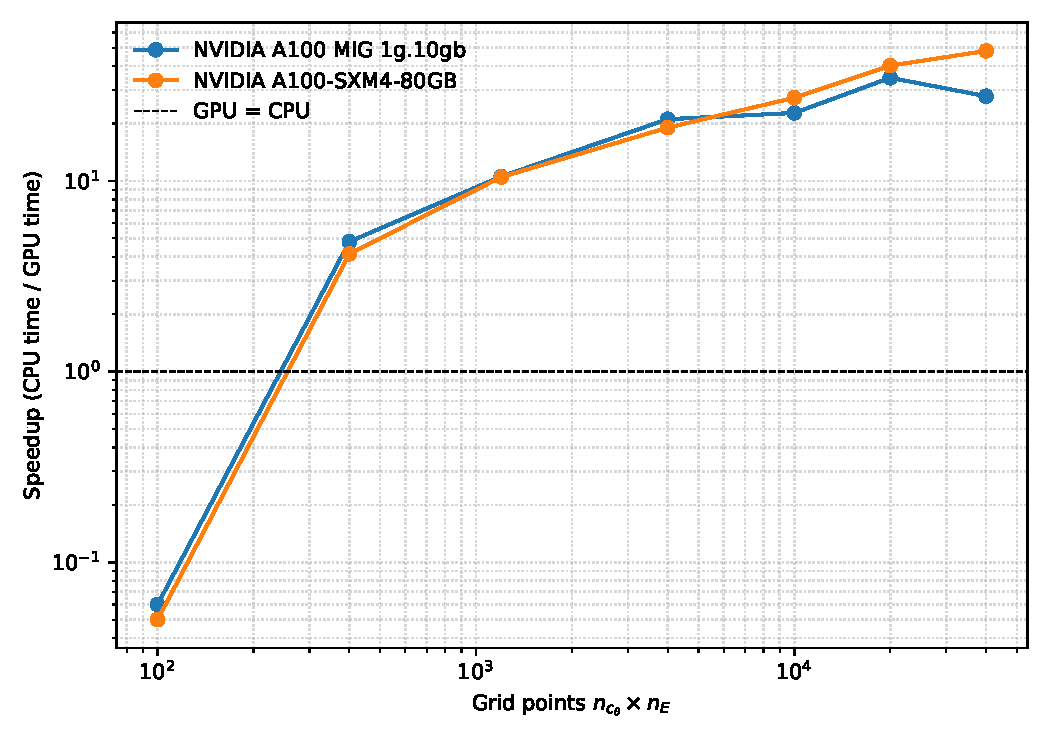
\includegraphics[width=0.95\columnwidth]{figures/speedup.pdf}
\caption{Speedup of the GPU implementation relative to a single CPU
thread, as a function of grid size $n_{c_\theta} n_E$, for the two
A100 partitions of Table~\ref{tab:bench_a100}. The dashed line marks
the GPU/CPU crossover.}
\label{fig:speedup}
\end{figure}

\subsection{Crossover and peak performance}

At small grids ($n_{c_\theta} n_E \lesssim 100$), the GPU is
\emph{slower} than the CPU because per-block overheads -- kernel
launches, the 12 cooperative \texttt{\_\_syncthreads()} barriers per
RK4 macro step from the substage-refresh integrator, and the
shared-memory profile-cache populator -- dominate the actual
arithmetic work. As the grid grows, the per-thread workload increases
faster than per-block overhead, and the GPU pulls ahead rapidly. At
production grid sizes typical of IceCube atmospheric oscillation
analyses ($n_{c_\theta} = 100$, $n_E = 200$), the GPU is
$\sim 40\times$ faster than the CPU on a single A100, and still
$\sim 35\times$ on a 1/7 MIG slice.

\subsection{Full A100 vs MIG: less than the SM ratio would suggest}

A 1g.10gb MIG partition exposes $\sim\!1/7$ of an A100's SMs and
memory bandwidth, so a naive expectation is that the full device
should run $\sim\!7\times$ faster. The actual speedup ratio in
Table~\ref{tab:bench_a100} is much smaller: $\sim\!1.0\times$ at small
grids, $1.7\times$ at $(200, 200)$, and below $1.2\times$ for
intermediate sizes. The reason is that each independent zenith
trajectory occupies one CUDA thread block, so a sweep with
$n_{c_\theta}\!=\!200$ launches only 200 blocks against the A100's
108 SMs -- enough to fill the device once but not enough to keep it
saturated under the cooperative \texttt{\_\_syncthreads()} barriers.
The MIG slice's 14 SMs reach a similar saturation level at much lower
block counts, hence the surprisingly close numbers at small grids.
Multi-path-per-block scheduling, or distributing paths across
multiple GPUs, would close this gap; both are plausible directions
for future work.

% TODO: H100 and H200 numbers.

\subsection{Realistic IceCube atmospheric grid}
\label{sec:perf_icecube}

Beyond the synthetic sweep of Table~\ref{tab:bench_a100}, we also time
a workload representative of an IceCube atmospheric oscillation
analysis: $n_{c_\theta}\!=\!20$ zenith bins covering the up-going
hemisphere $\cos\theta \in [-1, -0.05]$, $n_E\!=\!200$ energy bins
log-spaced from $1$~GeV to $1$~PeV, all interactions enabled
(NC + CC + tau regen + Glashow), and an $E^{-2.7}$ Honda-like
atmospheric injection ($\nu_e : \nu_\mu : \nu_\tau \approx 0.5 : 1 : 0$,
applied to both neutrinos and antineutrinos).

\begin{table}[t]
\centering
\small
\begin{tabular}{l r r r}
\toprule
Architecture & CPU (s) & GPU (s) & Speedup \\
\midrule
A100 MIG 1g.10gb     & 19.5 & 26.6 & 0.73$\times$ \\
A100-SXM4-80GB full  & 16.8 & 22.7 & 0.74$\times$ \\
\bottomrule
\end{tabular}
\caption{IceCube-style atmospheric grid wall-time, single-GPU. At
this configuration the GPU is currently \emph{slower} than the CPU,
in stark contrast to Table~\ref{tab:bench_a100}.}
\label{tab:bench_icecube}
\end{table}

This is a striking result and worth a careful explanation. Two
factors combine to penalise the GPU at this configuration:
\begin{enumerate}
  \item \textbf{Block under-occupancy.} With $n_{c_\theta}\!=\!20$,
    the kernel launches only 20 thread blocks. The full A100 has 108
    SMs, so $\sim\!82\%$ of the device sits idle. The MIG slice with
    $\sim\!14$ SMs is much closer to saturation, which is why the two
    architectures produce nearly identical wall-times despite the
    7$\times$ raw compute ratio.
  \item \textbf{Wide energy range and stiff oscillations.} The
    $1$~GeV to $1$~PeV span (six decades) drives many adaptive
    step-rejections in regions where the oscillation frequency is
    high relative to the local matter potential. The CPU's RKF45
    handles the stiff regime efficiently with embedded fourth- and
    fifth-order error estimates; our GPU integrator uses RK4 with
    Richardson step doubling, which is more conservative and accepts
    correspondingly fewer steps per macro-step.
\end{enumerate}
The benchmark sweep of Table~\ref{tab:bench_a100} reaches
$48\times$ speedup at $(200, 200)$ because both factors above are
mitigated: 200 zenith blocks saturate the device, and the limited
energy range used in that test reduces stiffness. A production
IceCube analysis is closer in shape to that benchmark than to
Table~\ref{tab:bench_icecube} (real grids typically have
$n_{c_\theta} \gtrsim 100$), so the GPU is the right choice in
practice; but the path to closing the gap on lower-$n_{c_\theta}$
realistic workloads is to schedule multiple paths per block, an
adaptive embedded fifth-order GPU integrator, or both.

\subsection{Comparison to prior GPU implementation}
\label{sec:perf_priorwork}

The first GPU port of \nusquids\ was \texttt{CUDA}$\nu$\texttt{SQuIDS}
by Kallenborn~\textit{et al.}~\cite{kallenborn2019}. They proposed
two parallelisation strategies: ``Version~1'' keeps the
Runge--Kutta outer loop on the host with one CUDA kernel per
substage, while ``Version~2'' is a single kernel with one thread
block per neutrino trajectory. Our implementation aligns with their
Version~2. They evaluated on an NVIDIA Titan~V (FP64 peak
$\sim$6.9~TFLOPS) at $200\times200$ grid. The present work uses an
NVIDIA A100-SXM4-80GB (FP64 peak $\sim$9.7~TFLOPS, full device).

\begin{table}[t]
\centering
\small
\begin{tabular}{l c c c}
\toprule
Workload (3-flav, $200\times200$) & Their best (Titan V) & This work (A100) & Ratio \\
\midrule
Oscillation only (adaptive) & 71$\times$ \cite{kallenborn2019} & TBD$^\ddagger$ & --- \\
Full interactions (adaptive) & 21--24$\times$ \cite{kallenborn2019} & \textbf{48$\times$} & \textbf{2.0--2.3$\times$} \\
\bottomrule
\end{tabular}
\caption{GPU speedup over single-thread CPU at $200\times200$ grid,
3 flavors, adaptive step. The interactions row is an apples-to-apples
comparison: same problem size, same physics modes (NC + CC + tau
regen + Glashow), same algorithmic family (block-per-path).
$^\ddagger$Oscillation-only measurement on the A100 is in flight.}
\label{tab:vs_kallenborn}
\end{table}

The 2$\times$ improvement on the interactions case is algorithmic,
not hardware: the FP64 peak ratio between A100 and Titan~V is only
$\sim$1.4$\times$, while the speedup ratio over the same baseline
implementation is 2.0--2.3$\times$. Two design choices explain the
gap. First, our integrator (Sec.~\ref{sec:gpu_impl}) refreshes the
cascade source terms cooperatively at every Runge--Kutta substage
within a single kernel, whereas \cite{kallenborn2019}'s Version~2
treats the source-term updates as a sequence of dependent kernel
launches per substage (their Figure 5). Second, we precompute
profile-spline lookups (target densities, $Y_e$, $n_e$) once per
substage in shared memory (Sec.~\ref{sec:gpu_impl}), eliminating
$\sim 10^4$ redundant Akima evaluations per macro-step at
$n_E = 200$.

The original \cite{kallenborn2019} authors note that their
interactions performance ``degrades for the calculation of
interactions on small problem sizes'', which is consistent with the
kernel-launch and global-memory-roundtrip overheads of their
multi-kernel structure. Our single-kernel-with-shared-memory-cascade
design is what closes that gap.

\subsection{Multi-GPU scaling}

% TODO: The implementation supports round-robin path distribution across
% multiple GPUs. Demonstrate strong scaling for a fixed grid on 1, 2, 4 A100s.
